\documentclass[tikz, margin=1in]{standalone}
\usepackage{ifthen}

\usetikzlibrary{calc, arrows.meta, bending, math}

\def\isLeft{1}
\def\isCw{1}
\def\centerOffset{1}

\tikzset{
    arc center/.is choice,
    arc center/left/.code={\def\isLeft{1}\tikzset{arc to}},
    arc center/right/.code={\def\isLeft{0}\tikzset{arc to}},
    arc center offset/.code={\def\centerOffset{#1}\tikzset{arc to}},
    arc direction/.is choice,
    arc direction/cw/.code={\def\isCw{1}\tikzset{arc to}},
    arc direction/ccw/.code={\def\isCw{0}\tikzset{arc to}},
    arc to/.style={
        to path={
            [evaluate={
                coordinate \u, \v, \m, \mv, \mvOrtho, \c, \cu, \cv;
                \u = (u);
                \v = (v);
                \m = (\u)!0.5!(\v);
                \mv = (\v)-(\m);
                if \isLeft then {
                    \mvOrtho = (-\mvy, \mvx);
                } else {
                    \mvOrtho = (\mvy, -\mvx);
                };
                \c = (\m)+(\mvOrtho);
                \c = (\m)!\centerOffset!(\c);
                \cu = (\u)-(\c);
                \cv = (\v)-(\c);
                \radius = veclen(\cu);
                \startAngle = atan2(\cuy, \cux);
                \endAngle = atan2(\cvy, \cvx);
                if \isCw then {
                    if \startAngle < \endAngle then {
                        \endAngle = \endAngle - 360;
                    };
                } else {
                    if \startAngle > \endAngle then {
                        \endAngle = \endAngle + 360;
                    };
                };
            }]
            arc[radius=\radius pt, start angle=\startAngle, end angle=\endAngle] \tikztonodes
        }
    }
}

\begin{document}
    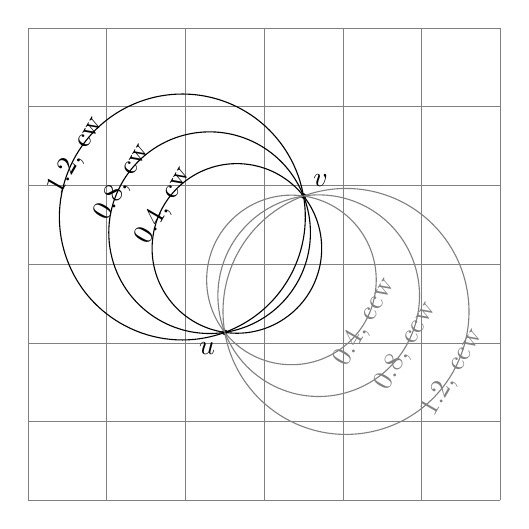
\begin{tikzpicture}[
            every circle/.style={radius=1pt},
            sloped
        ]
        \draw[help lines] (0, 0) grid (6,6);

        \path[shift={(3,3)}, rotate=-30] 
            coordinate (u) at (0, -1)
            coordinate (v) at (0, 1);
        
        \fill (u) circle node[below left] {\(u\)};
        \fill (v) circle node[above right] {\(v\)};

        \foreach \i in {0.4, 0.8, 1.2} {
            \draw (u) 
                to[arc center=left, arc direction=cw, arc center offset=\i]
                node{\i, cw} (v);

            \draw (u) 
                to[arc center=left, arc direction=ccw, arc center offset=\i]
                (v);

            \draw[color=gray] (u) 
                to[arc center=right, arc direction=ccw, arc center offset=\i]
                node{\i, ccw} (v);

            \draw[color=gray] (u) 
                to[arc center=right, arc direction=cw, arc center offset=\i]
                (v);

        }
    \end{tikzpicture}
\end{document} 